We start our investigation by determining the work output $W$ when varying the time between qubit switching $\Delta t$.
If the System qubit is initialised in the pure state $\rho_S = \ket{0} \bra{0}$, the work output for a single jump is given by (see appendix \ref{deriv_jump} for a derivation)
\begin{equation} \label{single_work}
	W = \frac{1}{\abs{\alpha}} sin(2\abs{\alpha}\Delta t) \Im{(\tau' - \tau) \alpha^*}
\end{equation}
\begin{equation*}
	\alpha = \frac{1}{2} \left[sin(\theta_D^1) e^{i\phi_D^1} + sin(\theta_T^1) e^{i\phi_T^1}\right], \\
	\tau' - \tau = \frac{1}{2} \left[ sin(\theta_T^2)e^{i\phi_T^2} - sin(\theta_T^1)e^{i\phi_T^1} \right].
\end{equation*}

From equation \ref{single_work} it becomes evident that for $\Delta t \to 0, W \to 0$. This is confirmed by the following where, for multiple values of $N$, we simulate 500 random Drive functions for each $\Delta t$ and find their optimal Transducer policy. The average work output over the 500 runs scaled by the amount of PWC steps $\overline{W}/N$ for 20 values of $\Delta t$ is shown in figure \ref{dt_dep}.

\begin{figure}
	\centering
	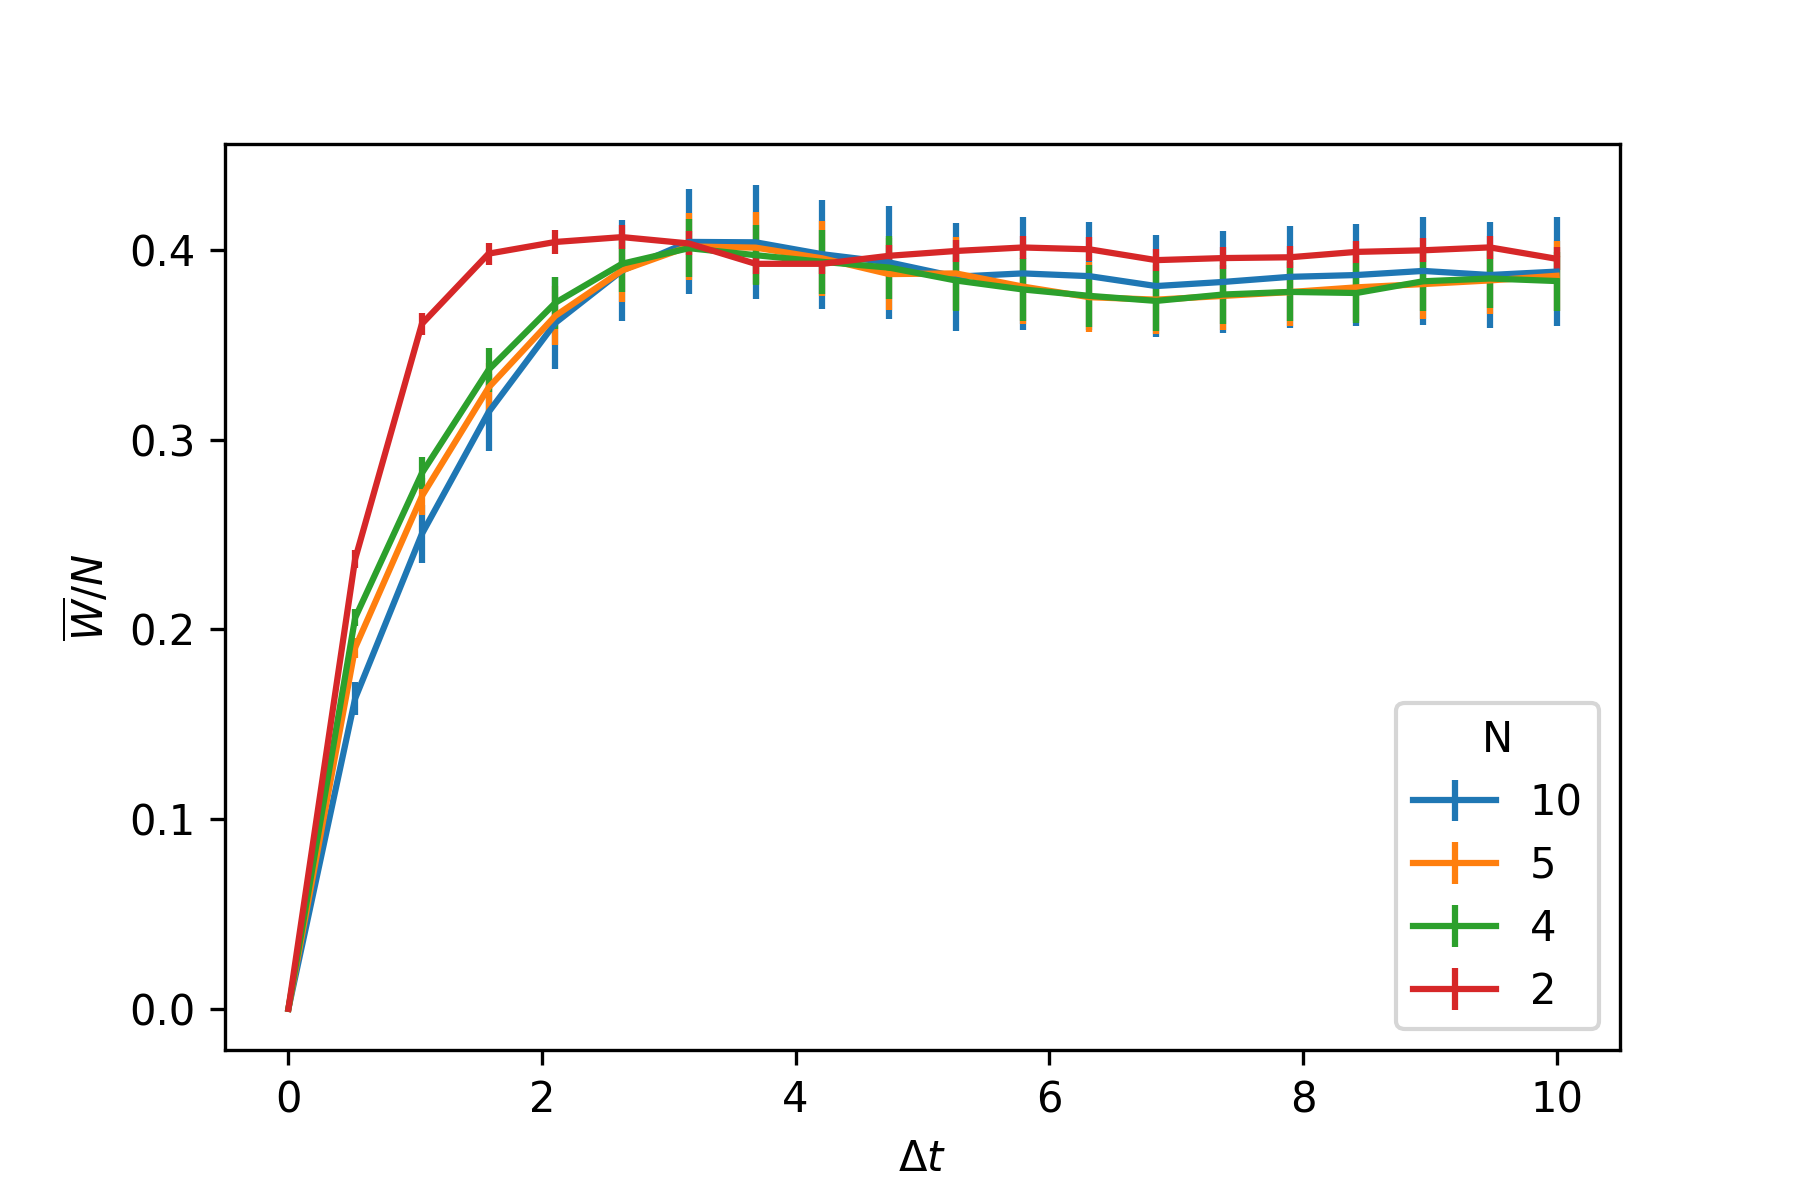
\includegraphics[width=0.7\textwidth]{img/dt_dep}
	\caption{We plot the average work $\overline{W}$ over 500 runs for random excitations divided by amount of PWC steps $N$, for all of which we use $\rho_0 = \ket{0}\bra{0}$. The error bars correspond to the standard deviation $\sigma_{\overline{W}}$.}
	\label{dt_dep}
\end{figure}